\subsection{Structural Analysis}

\label{sec:structural}

Structural analysis studies the interrelation between parameters and variables of the system by establishing constraints. The constraints can be obtained from the equations describing the system model. Structural analysis distinguishes known and unknown variables, according to whether they can be measured or not. Then the unknown variables are expressed using the known ones, using the constraints. Structural analysis based residual signal generation requires that unknown variables can be expressed redundantly. One of the constraints is used to express the unknown, the other to verify it. If there's a mismatch between the two, a fault is detected.

When looking for sensor faults, one constraint is between the measured and the actual values of a variable. When a sensor fault occurs, there can be a considerable difference between the measured and the actual value of a variable. Assuming that only one fault occurs at any given time, faults cannot mutually neutralize each other. The following structural analysis based residual generator is able to detect both actuator and sensor faults.

The constraints being used to detect faults in the motor are derived from the equations in section \ref{sec:motors} and are listed in equations \ref{eq:const1} to \ref{eq:const4}. $C_i$ represents constraint relations, $d_i$ represent differential relations. The relation between the constraints and the variables are illustrated by figure \ref{fig:structDiagram}.

%\begin{figure}
%	\centering
%	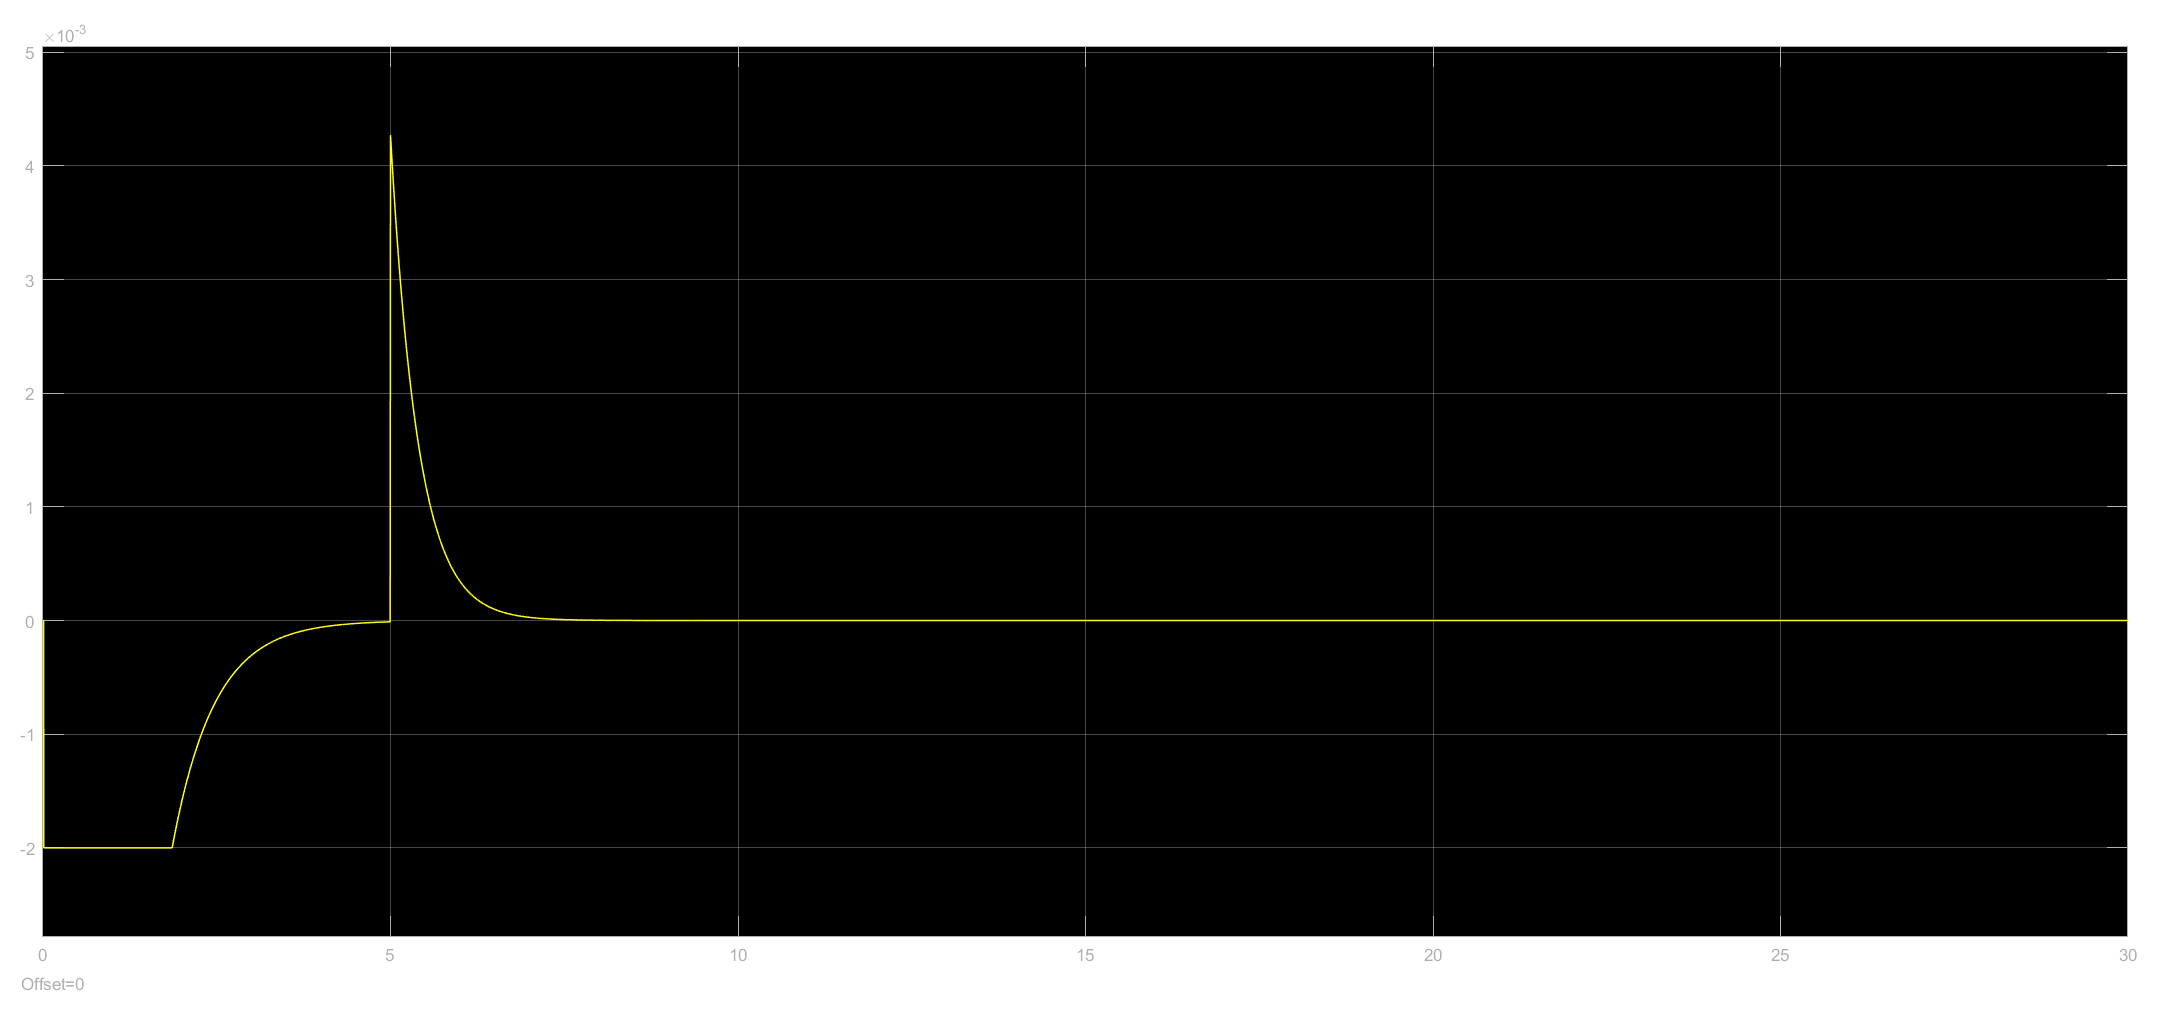
\includegraphics[width=120mm]{figures/rwFaultTorque}
%	\caption{Torque jump in scenario where at 5s the reaction wheel friction doubles}
%	\label{fig:rwFaultTorque}
%\end{figure} 


%\begin{figure}
%	\centering
%	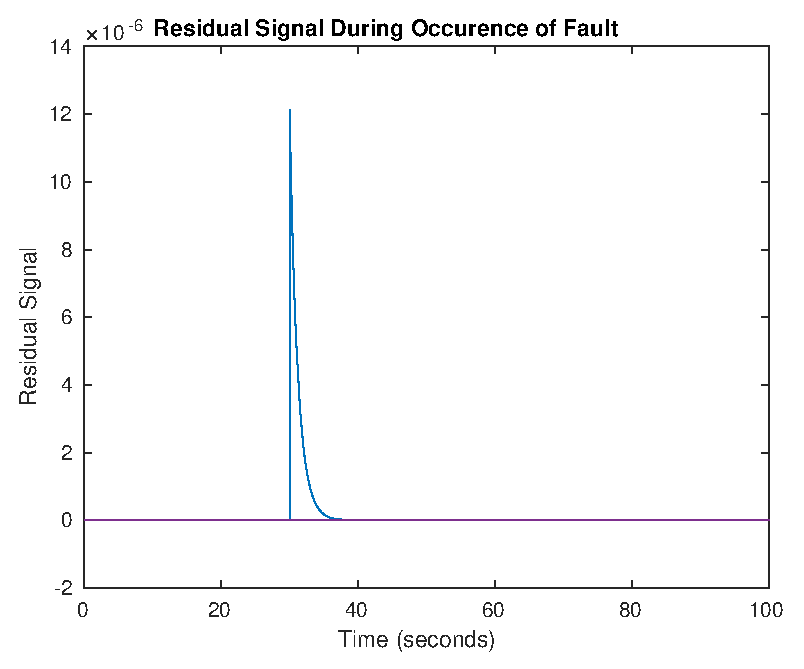
\includegraphics[width=120mm]{figures/residual}
%	\caption{Insert caption}
%	\label{fig:residual}
%\end{figure} 
%

%
%\begin{figure}
%	\centering
%	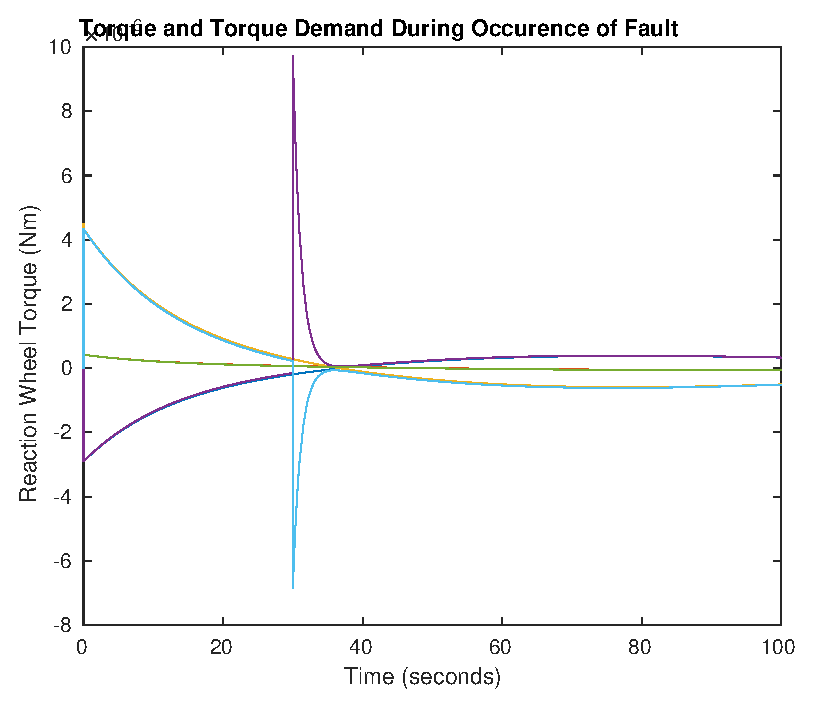
\includegraphics[width=120mm]{figures/residTau}
%	\caption{Insert caption}
%	\label{fig:residualTau}
%\end{figure} 

\begin{equation}
C_1(\omega, v) = V_a = R_a i + k_e \omega
\label{eq:const1}
\end{equation}

\begin{equation}
C_2(\omega, \dot{\omega}, i) =  k_{t}i  =J\dfrac{d\omega}{dt} + b\omega
\label{eq:const2}
\end{equation}

\begin{equation}
C_2(\tau, i) = \tau = k_t i
\label{eq:const3}
\end{equation}
\todo{adjust to right tau}
\begin{equation}
d_1(\omega, \dot{\omega})
\label{eq:const4}
\end{equation}


\begin{figure}[h]
	\centering
	\begin{tabular}{@{}c@{\hspace{.5cm}}c@{}}
		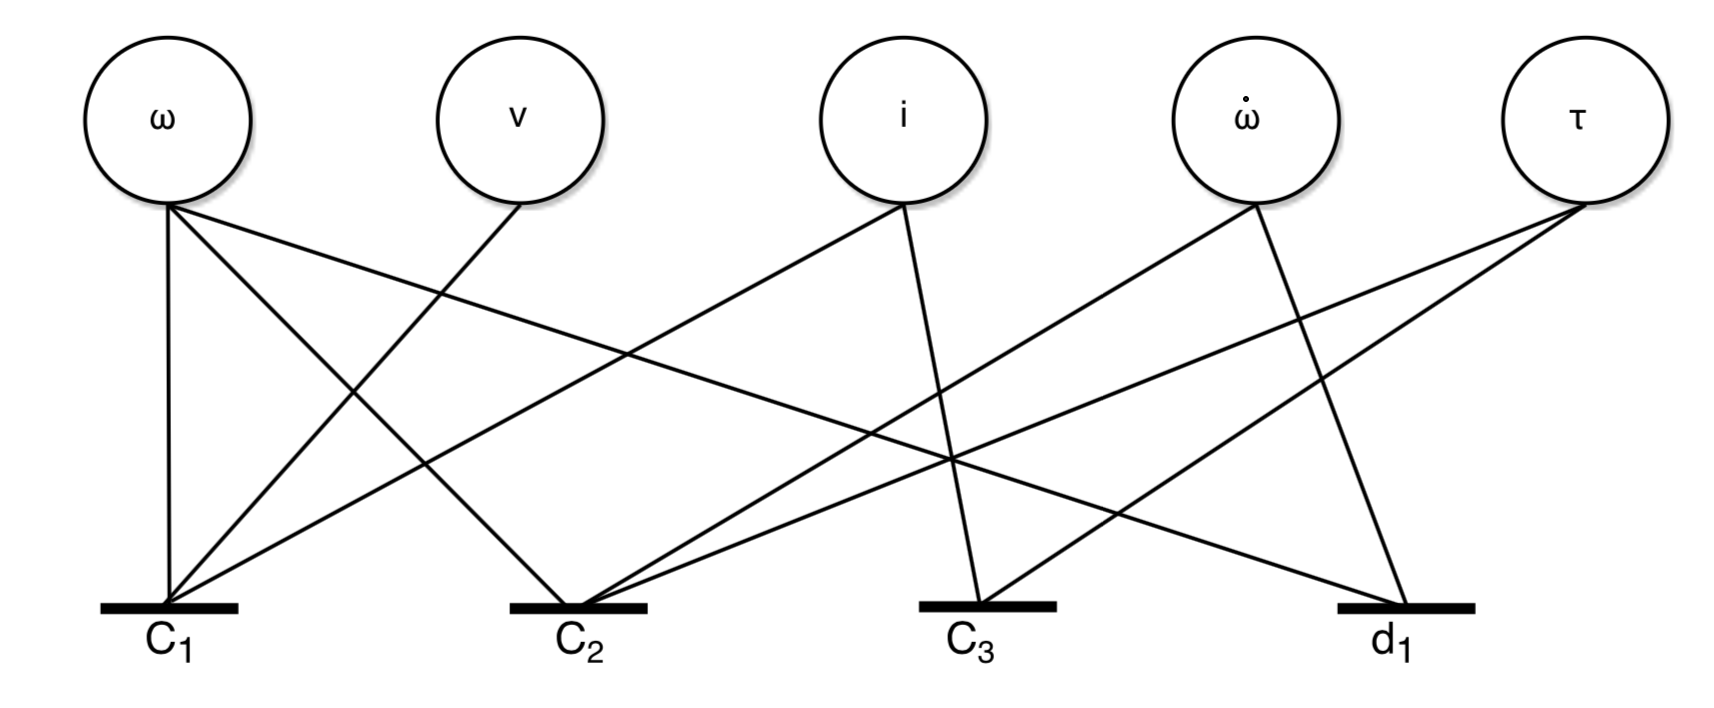
\includegraphics[page=1,width=1\textwidth]{fault_diagram}
	\end{tabular}
	\caption{Structural graph of reaction wheel motor}
	\label{fig:structDiagram}
\end{figure}


$\omega$ and $i$ can be measured, so the residual signal can be derived according to \ref{eq:res1}. In absence of fault, the residual should be close to zero.

\begin{equation}
residual = k_t i + J \frac{d\omega}{dt} + b \omega
\label{eq:res1}
\end{equation}

The friction model is quite accurate at high speeds, not so much for low speeds. This needs to be addressed by a higher threshold fault signal threshold at low speeds. Figures \ref{fig:residual} - \ref{fig:residualOmega} show the effect of a bearing fault on the residual. The fault doubles the reaction wheel friction.

 When a residual indicates a fault, the torque distributor changes mode, shutting down the faulty wheel. There's a short term error in the reaction wheel subsystem's torque output, but then the torque reference tracking normalizes quite quickly. This might jeopardize a downlink operation, but since this kind of fault rarely occurs, the effects are not serious. \todo{move}


\begin{figure}[h]
	\centering
	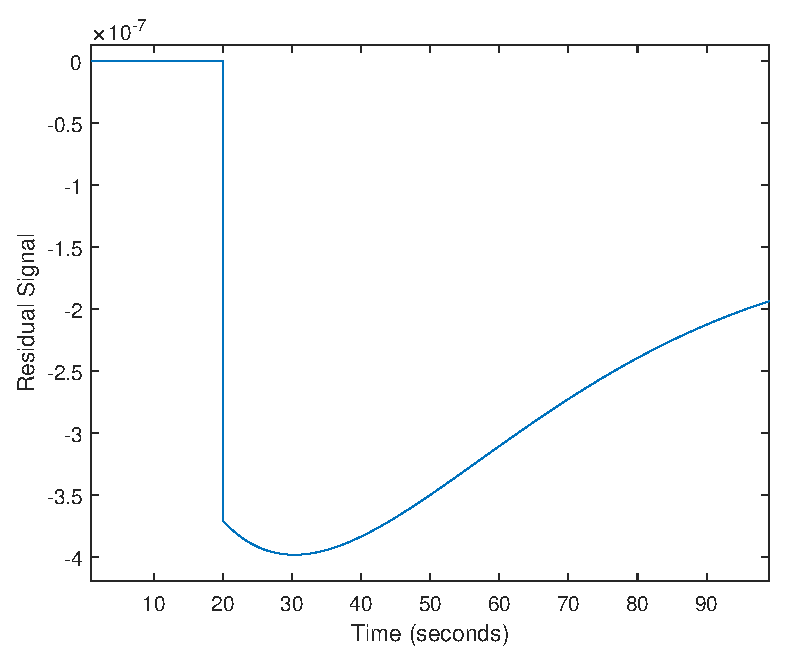
\includegraphics[width=120mm]{figures/residual_Noreconfig}
	\caption{Residual signal in scenario where at 20 s the reaction wheel friction doubles}
	\label{fig:residual}
\end{figure} 

\begin{figure}[H]
	\centering
	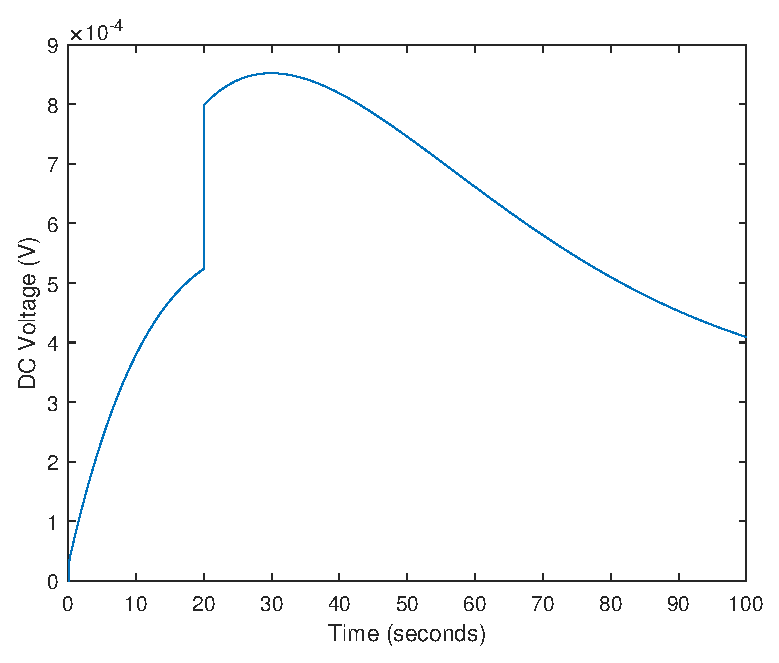
\includegraphics[width=120mm]{figures/voltage_Noreconfig}
	\caption{DC control voltage signal of angular velocity controlled reaction wheel in scenario where at 20 s the reaction wheel friction doubles}
	\label{fig:rwFaultRes3}
\end{figure} 

\begin{figure}[h]
	\centering
	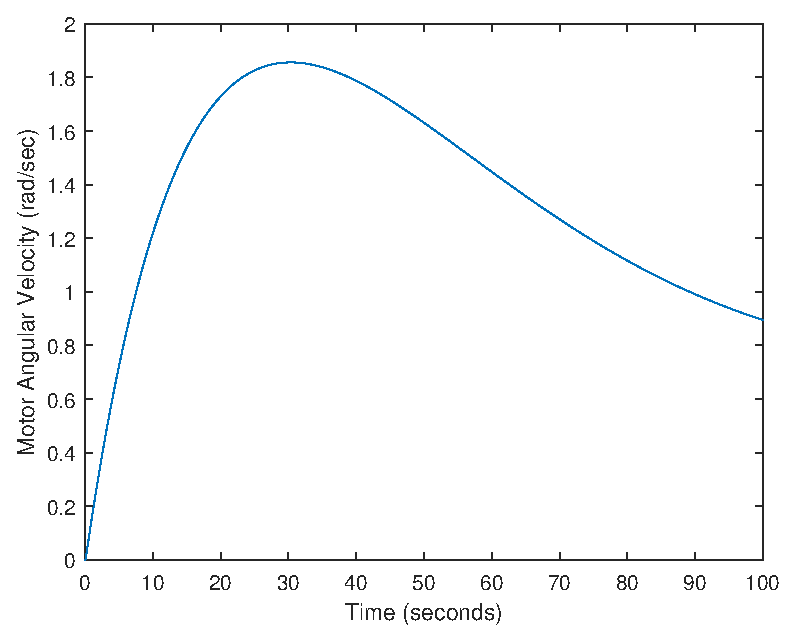
\includegraphics[width=120mm]{figures/omega_Noreconfig}
	\caption{Angular velocity in scenario where at 20 s the reaction wheel friction doubles}
	\label{fig:residualOmega}
\end{figure} 


%\section{Alternative method for identifying reaction wheel fault}
%
%With enough computational power the faulty reaction wheel can be detected through the calculated reaction wheel output torque, assuming only one reaction wheel is faulty. It is done by calculating the difference between 3D torque demand and actual 3D torque output. 
%
%\begin{equation}
%\vec{N}_{rw} = \underline{I}_s \dot{\vec{\omega}}  + \vec{\omega} \times \vec{h_{rw}} - \vec{N_{mt}} - \vec{N_{dist}}
%\end{equation}
%
%Then the difference between torque demand and torque output is calculated. The reaction wheel that has the most similar axis orientation to the torque difference is deemed as faulty.
%
%\begin{equation}
%\vec{N}_{rw}^{demand} - \vec{N}_{rw}^{actual} = 
%\vec{N}_{rw}^{diff}
%\end{equation}
%
%\begin{equation}
%\pm \vec{N}_{rw}^{diff}  \stackrel{?}{\approx} \vec{axis} 
%\end{equation}
%
%If the torque error exceeds a certain threshold, then the faulty wheel index can be identified as
%
%unit vectors!!!
%
%\begin{equation}
%faultyWheelIndex = \arg\min_i ( \pm \vec{N}_{rw}^{diff} - \vec{axis}_i ) 
%\end{equation}
%
%\todo{mention unit vector notation, decide notation for axis, express axis according to q}
%
%Note: the lag for torque change and wheel saturation has to be taken into account separately, as those don't count as faults. 
%Thresholds should be applied.